%\documentclass{article}
%\usepackage{amsmath, amssymb, amsthm}
%\usepackage[utf8]{inputenc} % 支持中文
%\usepackage[UTF8]{ctex}
%\usepackage{xcolor}
%\usepackage{tcolorbox}
%\usepackage{fancyhdr} % 设置页眉页脚
%\usepackage{tikz}
%\usepackage{geometry}
%\usepackage{algorithm}
%\usepackage{algorithmic}
%\usepackage{titlesec}
%\geometry{a4paper, margin=2cm}
%% 定义色彩方案
%\definecolor{shadecolor}{rgb}{0.95, 0.95, 1}
%\definecolor{theoremboxcolor}{rgb}{0.9, 0.95, 1}
%\definecolor{algboxcolor}{rgb}{1.0, 0.92, 0.8}
%% 设置页眉
%\pagestyle{fancy}
%\fancyhf{}
%\lhead{\textbf{Kenan Xu}}
%\rhead{\textbf{学海无涯}}
%\renewcommand{\headrulewidth}{0.4pt}
%\renewcommand{\footrulewidth}{0pt}
%% 美化标题
%%\titleformat{\section}{\Large\bfseries\color{blue}}{\thesection}{1em}{}
%%\titleformat{\subsection}{\large\bfseries\color{teal}}{\thesubsection}{1em}{}
%% 定理环境美化
%\newtcolorbox{mytheorem}[1][]{colback=theoremboxcolor, colframe=blue!75!black, title=定理, #1}
%\newtcolorbox{mydefinition}[1][]{colback=theoremboxcolor, colframe=blue!75!black, title=定义, #1}
%\newtcolorbox{myproposition}[1][]{colback=theoremboxcolor, colframe=blue!75!black, title=命题, #1}
%\newtcolorbox{myshadedbox}[1][]{colback=shadecolor, colframe=black!50, #1}
%\newtcolorbox{myalgorithm}[1][]{colback=algboxcolor, colframe=orange!85!black, title=算法, #1}
%% 定理、定义、引理和命题的定义
%\newtheorem{theorem}{定理}
%\newtheorem{definition}{定义}
%\newtheorem{lemma}{引理}
%\newtheorem{proposition}{命题}
%\begin{document}
%	\begin{center}
%		{\LARGE \textbf{标题}}
%	\end{center}
%	\section*{引言}
%	% 引言部分内容
%	\section*{基本思想}
%	% 基本思想部分内容
%	\section*{几何解释}
%	\begin{myshadedbox}
%		% 几何解释的内容
%	\end{myshadedbox}
%	\begin{center}
%		\begin{tikzpicture}[scale=1]
%			% 在此处添加图示
%		\end{tikzpicture}
%	\end{center}
%	\section*{算法介绍}
%	\begin{myalgorithm}
%		\begin{algorithm}[H]
%			\caption{算法名称}
%			\begin{algorithmic}[1]
%				\STATE 初始化参数
%				\FOR{循环条件}
%				\STATE 计算某些值
%				\IF{条件}
%				\STATE 做一些事情
%				\ENDIF
%				\ENDFOR
%			\end{algorithmic}
%		\end{algorithm}
%	\end{myalgorithm}
%	\section*{收敛性分析}
%	\begin{mytheorem}
%		% 定理的描述和内容
%	\end{mytheorem}
%	\begin{proof}
%		% 定理的证明过程
%	\end{proof}
%	\section*{方法比较}
%	\begin{myshadedbox}
%		% 对不同方法的比较内容
%	\end{myshadedbox}
%	\section*{应用与案例分析}
%	% 应用和案例分析的内容
%	\subsection*{案例：某某模型拟合}
%	% 详细的案例分析内容
%	\section*{总结}
%	\begin{tcolorbox}[colback=yellow!5!white, colframe=yellow!75!black]
%		% 总结部分的内容
%	\end{tcolorbox}
%\end{document}


%Latex 模板 2
\documentclass[a4paper, 12pt]{report}
\usepackage{amsmath, amsfonts, amssymb, amsthm}
\usepackage[utf8]{inputenc} % 支持中文
\usepackage[UTF8]{ctex}
\usepackage{geometry}
\usepackage{xcolor}
\usepackage{tcolorbox}
\usepackage{fancyhdr}
\usepackage{algorithm}
\usepackage{algpseudocode}
\usepackage{hyperref}
\usepackage{graphicx}
\usepackage{titlesec}
\usepackage{xcolor} 
\usepackage{float}
\usepackage{framed}
\usepackage{fancyhdr}
\usepackage{booktabs}
%%%%%%%%%%%%%%%%%%%%%Definition for Math Form %%%%%%%%%%%%%%%%%%%%%%%%%%%%%%%%%%%%
\def\[{\begin{equation*}}
\def\]{\end{equation*}}
\def\lb{\left(}
\def\rb{\right)}
\def\lno{\left\|}
\def\rno{\right\|}
\def\lbb{\left\{}
\def\rbb{\right\}}
\def\lzb{\left[}
\def\rzb{\right]}
\def\lang{\left\langle}
\def\rang{\right\rangle}
\def\argmin{\arg\min}
\def\argmax{\arg\max}
\def\shrink{{\rm shrink}}
\def\prox{{\rm \bf prox}}
\def\I{{\rm \bf I}}

\def\be{\beta}
\def\si{\sigma}
\def\lam{\lambda}
\def\tlam{\widetilde\lam}
\def\blam{\bar\lam}
\def\hlam{\widehat\lam}
\def\tM{{\widetilde M}}

\def\nn{\nonumber}
\def\st{\hbox{s.t.}}
\def\t{\top}

\def\a{{\bm a}}
\def\b{{\bm b}}
\def\c{{\bm c}}
\def\d{{\bm d}}
\def\F{{\mathbf{F}}}
\def\B{{\mathcal B}}
\def\C{{\mathcal C}}
\def\L{{\mathcal L}}
\def\Q{{\mathcal Q}}
\def\P{{\mathcal P}}
\def\R{{\mathbb R}}
\def\S{{\mathcal S}}
\def\u{{\bm u}}
\def\v{{\bm v}}
\def\x{{\bm x}}
\def\tx{{\widetilde \x}}
\def\y{{\bm y}}
\def\ty{{\widetilde \y}}
\def\Z{{\mathcal Z}}
\def\z{{\bm z}}
\def\W{{\mathcal W}}
\def\w{{{\bm w}}}
\def\tw{{\widetilde \w}}
\def\tu{{\widetilde \u}}
\def\q{{{\bm q}}}
%%%%%%%%%%%%%%%%%%%%%%%%%%%%%%%%%%%%%%%%%%%%%%%%%%%%%%%%%%%%%%%%%%%%%%%%%%%%%%%%
% 设置页面布局
\geometry{a4paper, left=2.2cm, right=2.2cm, top=2.5cm, bottom=3cm}
\setlength{\headsep}{0.75in}
% 定义色彩方案
\definecolor{shadecolor}{rgb}{0.85, 0.95, 1} 
\definecolor{theoremboxcolor}{rgb}{0.9, 0.95, 1}
\definecolor{remarkboxcolor}{rgb}{1.0, 0.92, 0.8}
\definecolor{hong}{RGB}{199,21,133}
\definecolor{huang}{RGB}{255,164,0}
\definecolor{analysisboxcolor}{rgb}{0.9, 0.9, 1}
% 设置页眉
\pagestyle{fancy}
\fancyhf{}
\fancyhead[L]{\textbf{AI4E}}
\fancyhead[R]{\textbf{Conanxu}}
% 设置页码显示
\fancyfoot[C]{\thepage} % 页码居中显示在页脚
\renewcommand{\headrulewidth}{0.4pt}
% 美化标题
\titleformat{\section}{\Large\bfseries\color{black}}{\thesection}{1em}{}
\titleformat{\subsection}{\large\bfseries\color{black}}{\thesubsection}{1em}{}
% 定理环境美化
\newtcolorbox{mytheorem}[1][]{colback=theoremboxcolor, colframe=blue!75!black, title=定理, #1}
\newtcolorbox{mydefinition}[1][]{colback=theoremboxcolor, colframe=blue!75!black, title=定义, #1}
\newtcolorbox{myproposition}[1][]{colback=theoremboxcolor, colframe=blue!75!black, title=命题, #1}
\newtcolorbox{myremark}[1][]{colback=remarkboxcolor, colframe=red!75!black,
title=Remark, #1}
\newtcolorbox{myalert}[1][]{colback=red!15, colframe=red!75!black}
\newtcolorbox{myanalysis}[1][]{colback=analysisboxcolor, colframe=blue!55!black, title=\textbf{Analysis}, fonttitle=\bfseries, #1}
% 算法框的美化
\newtcolorbox{myalgorithm}[1][]{colback=remarkboxcolor, colframe=orange!85!black, title=算法, #1}
% 定理环境
\newtheorem{theorem}{定理}[section]
\newtheorem{definition}{定义}[section]
\newtheorem{lemma}{引理}[section]
\newtheorem{proposition}{命题}[section]
\newtheorem{corollary}{推论}[section]
\newtheorem{remark}{备注}[section]
\newtheorem{exer}{练习}[section]
\newtheorem{que}{问题}[section]
\newtheorem{example}{示例}[section]
\newtheorem{property}{性质}[section]
\newcommand{\alert}[1]{\textcolor{red}{\textbf{#1}}}
%封面
\makeatletter
\renewcommand*{\maketitle}{
\begin{titlepage}
%		\pdfbookmark[1]{Cover}{cover}
\centering
%\scshape
\vspace*{5\baselineskip}
%		\color{hong}

%----- title -----
\rule{\textwidth}{1.6pt}\vspace*{-\baselineskip}\vspace*{2pt}
\rule{\textwidth}{0.4pt}

\vspace{0.75\baselineskip}

{\LARGE\bfseries \@title}

\vspace{0.75\baselineskip}

\rule{\textwidth}{0.4pt}\vspace*{-\baselineskip}\vspace{3.2pt}
\rule{\textwidth}{1.6pt}

\vspace{4\baselineskip}

%----- Author -----
{\Large \@author}

\vspace{0.35\baselineskip}	

%----- Date -----
{\Large \@date}
\vfill
\end{titlepage}
}
\makeatother
\title{学海无涯苦作舟 \\[20pt]
\Large 
}
\author{洗衣机}
%\institute{}
%\version{1.3}
%\date{\zhtoday}
\date{Last Update: \today}
\begin{document}
\maketitle
\clearpage
% 目录页不显示页码
\pagenumbering{gobble}  % 禁用页码显示
\tableofcontents  % 生成目录
% 重新启用页码，从 1 开始
\clearpage
\pagenumbering{arabic}
\chapter{Optimizaiton}
\section{概念$\&$定义}
\begin{definition}[凸函数]\label{def:convex}
	令 $\Omega\subset\mathbb R^n$ 为凸集，$\theta:\Omega\to\mathbb R$。若对任意 $u,v\in\Omega$ 和 $\lambda\in[0,1]$，都有
	\[
	\theta\bigl(\lambda u + (1-\lambda) v\bigr)
	\le \lambda\,\theta(u) + (1-\lambda)\,\theta(v),
	\]
	则称 $\theta$ 在 $\Omega$ 上为\emph{凸函数}。
\end{definition}

\begin{definition}[严格凸函数]
	在同样记号下，若对任意 $u,v\in\Omega$ 且 $u\neq v$，以及 $\lambda\in(0,1)$，严格不等式
	\[
	\theta\bigl(\lambda u + (1-\lambda) v\bigr)
	< \lambda\,\theta(u) + (1-\lambda)\,\theta(v)
	\]
	成立，则称 $\theta$ 在 $\Omega$ 上为\emph{严格凸函数}。
\end{definition}

\begin{definition}[强凸函数]
	若存在常数 $\sigma>0$，使得对任意 $u,v\in\Omega$ 和 $\lambda\in(0,1)$，
	\[
	\theta\bigl(\lambda u + (1-\lambda) v\bigr)
	\le \lambda\,\theta(u) + (1-\lambda)\,\theta(v)
	- \frac{\sigma}{2}\,\lambda(1-\lambda)\,\|u-v\|^2,
	\]
	则称 $\theta$ 在 $\Omega$ 上为\emph{强凸函数}。
\end{definition}

\begin{remark}
	由上述定义可知：
	\[
	\text{强凸}\;\Longrightarrow\;\text{严格凸}\;\Longrightarrow\;\text{凸}.
	\]
\end{remark}

\begin{definition}[可微凸函数的梯度不等式]
	若 $\theta$ 在 $\Omega$ 上可微，则对任意 $u,v\in\Omega$ 有
	\[
	\theta(u)\ge \theta(v) + \nabla\theta(v)^{T}(u-v)
	\]
	当且仅当 $\theta$ 为凸函数。
\end{definition}

\begin{definition}[次梯度与次微分]
	令 $\theta:\Omega\to\mathbb R$，$\Omega$ 凸。若对于某向量 $s\in\mathbb R^n$，对任意 $u\in\Omega$，都有
	\[
	\theta(u)\ge \theta(v) + s^{T}(u-v),
	\]
	则称 $s$ 为 $\theta$ 在 $v\in\Omega$ 处的\emph{次梯度}（Subgradient）。所有次梯度构成的集合称为 $\theta$ 在 $v$ 处的\emph{次微分}（Subdifferential），记为 $\partial\theta(v)$。
\end{definition}

\begin{definition}[Lipschitz 连续]
	令 $F:\Omega\to\mathbb R^m$。若存在常数 $L>0$，使得对所有 $u,v\in\Omega$，
	\[
	\|F(u)-F(v)\|\le L\,\|u-v\|,
	\]
	则称 $F$ 在 $\Omega$ 上为\emph{Lipschitz 连续}（Lipschitz continuous）。
\end{definition}

\begin{definition}[算子类型]\label{def:operator-types}
	令 $\Omega\subset\mathbb R^n$ 为凸集，$F:\Omega\to\mathbb R^n$ 为映射；亦令 $(\mathcal{H},\|\cdot\|)$ 为实 Hilbert 空间，$T:\mathcal{H}\to\mathcal{H}$。则：
	
	\begin{enumerate}
		\item （单调算子 Monotone）若对任意 $u,v\in\Omega$ 有
		\[
		(u-v)^\top\bigl[F(u)-F(v)\bigr]\ge0,
		\]
		则称 $F$ 在 $\Omega$ 上为单调算子；
		
		\item （严格单调算子 Strictly Monotone）若对任意 $u,v\in\Omega,\ u\neq v$ 有
		\[
		(u-v)^\top\bigl[F(u)-F(v)\bigr]>0,
		\]
		则称 $F$ 为严格单调算子；
		
		\item （强单调算子 Strongly Monotone）若存在 $\eta>0$ 使得对任意 $u,v\in\Omega$，
		\[
		(u-v)^\top\bigl[F(u)-F(v)\bigr]\ge \eta\|u-v\|^2,
		\]
		则称 $F$ 为强单调算子；
		
		\item （伪单调算子 Pseudo–monotone）若对任意 $u,v\in\Omega$，
		\[
		(u-v)^\top F(v)\ge0
		\;\Longrightarrow\;
		(u-v)^\top F(u)\ge0,
		\]
		则称 $F$ 为伪单调算子；
		
		\item （余强制算子 Co–coercive）若存在 $\mu>0$ 使得对任意 $u,v\in\Omega$，
		\[
		(u-v)^\top\bigl[F(u)-F(v)\bigr]\ge \mu\|F(u)-F(v)\|^2,
		\]
		则称 $F$ 为余强制算子；
		
		\item （非扩张算子 Nonexpansive）若对任意 $x,y\in\mathcal{H}$ 有
		\[
		\|T(x)-T(y)\|\le \|x-y\|,
		\]
		则称 $T$ 为非扩张算子；
		
		\item （严格非扩张算子 Strictly Nonexpansive）若存在 $\rho\in[0,1)$ 使得对任意 $x,y\in\mathcal{H}$，
		\[
		\|T(x)-T(y)\|\le \rho\,\|x-y\|,
		\]
		则称 $T$ 为严格非扩张算子；
		
		\item （$\alpha$-平均算子 $\alpha$-Averaged）若存在 $\alpha\in(0,1)$ 与非扩张算子 $N$ 使得
		\[
		T = (1-\alpha)\,I + \alpha\,N,
		\]
		则称 $T$ 为 $\alpha$-平均算子。
	\end{enumerate}
\end{definition}
\newpage
\section{分式规划 (Fractional Programming): Dinkelbach 算法}
考虑如下问题
\[
\min_{x\in \S} F(x) = \frac{f(x)}{g(x)}
\]	
其中$f(x), g$ 是适当的闭凸函数, $g(x) > 0. $
\begin{shaded}
\begin{algorithm}[H]
\caption{Dinkelbach 算法}
\begin{algorithmic}[1]
%			\Require 目标函数 \( f(x) \)，约束条件 \( x \in X \)，精度阈值 \( \epsilon > 0 \)
%			\Ensure 最优解 \( x^* \) 和最优值 \( \lambda^* \)
\State \textbf{Input:} 初始值 \( \lambda^{(0)} \in \mathbb{R} \), 迭代次数 \( k = 0 \), 约束条件 \( x \in \S \), 精度阈值 \( \epsilon > 0 \)
\State \textbf{Output:} 最优解 \( x^* \) 和最优值 \( \lambda^* \)
\Repeat
\State \textbf{Step 1:} 求解子问题：
\[
x^{(k)} = \arg \max_{x \in X} \bigl\{ f(x) - \lambda^{(k)} g(x) \bigr\}
\]
\State \textbf{Step 2:} 计算：
\[
\phi(\lambda^{(k)}) = \max_{x \in X} \bigl\{ f(x) - \lambda^{(k)} g(x) \bigr\}
\]
\State \textbf{Step 3:} 更新：
\[
\lambda^{(k+1)} = \frac{f(x^{(k)})}{g(x^{(k)})}
\]
\State 更新迭代次数： \( k \gets k + 1 \)
\Until \( \phi(\lambda^{(k)}) < \epsilon \)
%			\State 输出最优解：\( x^* = x^{(k)} \)，最优值：\( \lambda^* = \lambda^{(k)} \)
\end{algorithmic}	
\end{algorithm}
\end{shaded}
\begin{property}
$\phi$ 关于$\lambda$ 单调递减: \(\lambda_1<\lambda_2\Rightarrow \phi(\lambda_1)>\phi(\lambda_2).\)
\end{property}
\begin{property}
$\lambda = \lambda^*\Leftrightarrow \phi(\lambda)=0.$ 
\begin{proof}
\begin{itemize} 
\item[$(\Rightarrow): $] 令$\lambda=\lambda^*=F(x^*)=\frac{f(x^*)}{g(x^*)}.$
$ \forall x \in \S, \lambda^*\leq \frac{f(x)}{g(x)}\Rightarrow f(x)-\lambda^*g(x)\geq 0$, 因此$x^*$恰好取到$\phi(\lambda^*)$的下界$0.$
\item[$(\Leftarrow):$] 假设存在$\lambda^\prime=F(x^\prime)$ 是更优解, 因此$\lambda^\prime=\frac{f(x^\prime)}{g(x^\prime)}<\lambda\Rightarrow f(x^\prime)-\lambda g(x^\prime)<0,$ \\$ \mathrm{i.e.} \phi(\lambda)<0, $矛盾.
\end{itemize}
\end{proof}
\end{property}
\section{酉不变性}
\begin{myalert}
酉矩阵保持内积不变
\end{myalert}
\begin{shaded}
\begin{itemize}
\item 酉矩阵保持向量范数不变;
\item 酉相似变换不改变矩阵的谱（特征值、奇异值）;
\end{itemize}
\end{shaded}
矩阵的F范数可以用奇异值刻画，因此也是酉不变的。

矩阵的诱导2范数等价于矩阵的谱半径，因此也是酉不变的。
\section{变分不等式}
\begin{shaded}
要证明变分不等式问题 \(\text{VI}(F, \mathbb{R}^n_+)\) 与互补问题  
\[
u \geq 0, \quad F(u) \geq 0, \quad u^T F(u) = 0
\]  
的等价性，我们需要分别证明两个方向的蕴含关系。

**1. 变分不等式 \(\Rightarrow\) 互补问题**
假设 \(u\) 是 \(\text{VI}(F, \mathbb{R}^n_+)\) 的解，即  
\[
\forall v \in \mathbb{R}^n_+, \quad (v - u)^T F(u) \geq 0.
\]  
需要证明 \(u\) 满足互补问题的三个条件。

**(1) 非负性 \(u \geq 0\) 和 \(F(u) \geq 0\)**
- 由于 \(\mathbb{R}^n_+\) 是可行域，显然 \(u \geq 0\)。
- 取 \(v = u + e_i\)（其中 \(e_i\) 是第 \(i\) 个单位向量），则 \(v \in \mathbb{R}^n_+\)，代入变分不等式得  
\[
(v - u)^T F(u) = e_i^T F(u) = F_i(u) \geq 0.
\]  
这对所有 \(i\) 成立，故 \(F(u) \geq 0\)。

**(2) 正交性 \(u^T F(u) = 0\)**
- 取 \(v = 0\)，代入变分不等式得  
\[
(0 - u)^T F(u) = -u^T F(u) \geq 0 \quad \Rightarrow \quad u^T F(u) \leq 0.
\]  
- 取 \(v = 2u\)，代入得  
\[
(2u - u)^T F(u) = u^T F(u) \geq 0.
\]  
- 结合两者，得 \(u^T F(u) = 0\)。

综上，\(\text{VI}(F, \mathbb{R}^n_+)\) 的解 \(u\) 满足互补问题。

---

**2. 互补问题 \(\Rightarrow\) 变分不等式**
假设 \(u\) 满足互补问题  
\[
u \geq 0, \quad F(u) \geq 0, \quad u^T F(u) = 0,
\]  
需要证明 \(u\) 是 \(\text{VI}(F, \mathbb{R}^n_+)\) 的解。

对任意 \(v \in \mathbb{R}^n_+\)，有  
\[
(v - u)^T F(u) = v^T F(u) - u^T F(u) = v^T F(u).
\]  
由于 \(v \geq 0\) 且 \(F(u) \geq 0\)，故 \(v^T F(u) \geq 0\)。因此  
\[
(v - u)^T F(u) \geq 0,
\]  
即 \(u\) 满足变分不等式。

---

**结论**
变分不等式 \(\text{VI}(F, \mathbb{R}^n_+)\) 和互补问题  
\[
u \geq 0, \quad F(u) \geq 0, \quad u^T F(u) = 0
\]  
在解集上完全等价。
\end{shaded}
\newpage
\section{凸的等价刻画}
\begin{shaded}
可微函数 $\theta(\cdot)$ 在非空凸集 $\Omega$ 上是凸的, 当且仅当其梯度 $\nabla\theta(\cdot)$ 是一个单调算子, 即对 $\nabla\theta(\cdot)$ 满足:

$$
(u-v)^T(\nabla\theta(u)-\nabla\theta(v)) \geq 0, \quad \forall u,\; v \in \Omega.
$$ 
\alert{证明关键在于将$\theta(u+t(u-v))$视作一元函数}

类似地, $\theta(\cdot)$ 是严格凸的等价于 $\nabla\theta(\cdot)$ 是严格单调的; $\theta(\cdot)$ 是强凸的等价于 $\nabla\theta$ 是强单调的. 但需要注意的是, 若一个映射 $F(\cdot)$ 是单调的, 我们并不能直接得到 $F(\cdot)$ 是某一凸函数 $\theta(\cdot)$ 的梯度; 其他情况也是类似的.
\end{shaded}
\newpage
\section{强凸函数的等价刻画}

设函数 $f : \mathbb{R}^n \to \mathbb{R}$，我们称 $f$ 是 $\mu$-强凸的（$\mu > 0$），若存在常数 $\mu > 0$，使得以下任一条件成立。若 $f$ 为连续可导函数，则下列条件等价：

\begin{enumerate}
	\item \textbf{一阶不等式形式（定义）}：对于任意 $x, y \in \mathbb{R}^n$，
	\[
	f(y) \ge f(x) + \langle \nabla f(x), y - x \rangle + \frac{\mu}{2} \|y - x\|^2.
	\]
	这是强凸性的经典定义形式，也称为带二次项的 Jensen 不等式。
	
	\item \textbf{梯度强单调性（gradient strong monotonicity）}：对于任意 $x, y \in \mathbb{R}^n$，
	\[
	\langle \nabla f(x) - \nabla f(y), x - y \rangle \ge \mu \|x - y\|^2.
	\]
	它反映了 $\nabla f$ 是 $\mu$-强单调的向量场。
	
	\item \textbf{Hessian 有界性（$f \in \mathcal{C}^2$ 时）}：
	\[
	\nabla^2 f(x) \succeq \mu I, \quad \forall x \in \mathbb{R}^n.
	\]
	即 $\nabla^2 f(x)$ 的最小特征值不小于 $\mu$，说明函数在每一点局部至少具有 $\mu$ 的曲率。
\end{enumerate}

\textbf{备注}：
\begin{itemize}
	\item 如果 $f$ 是不可微但闭凸函数，则强凸性的定义可通过次梯度推广为：
	\[
	f(y) \ge f(x) + \langle g, y - x \rangle + \frac{\mu}{2} \|y - x\|^2, \quad \forall x,y,\; g \in \partial f(x).
	\]
	\item 函数 $f$ 是 $\mu$-强凸的 $\Leftrightarrow$ 函数 $f(x) - \frac{\mu}{2} \|x\|^2$ 是凸的。
\end{itemize}

这些等价刻画为分析梯度法与一阶方法提供了理论基础。

\newpage
\section{理论依据：一阶条件下梯度下降为何一定下降？}
\begin{definition}[下降方向]
设 $f: \mathbb{R}^n \rightarrow \mathbb{R}$ 是定义在 $\mathbb{R}^n$ 上的连续可微函数。如果向量 $0 \neq \mathbf{d} \in \mathbb{R}^n$ 在点 $\mathbf{x}$ 处的函数 $f$ 的方向导数 $f'(\mathbf{x}; \mathbf{d})$ 是负的，即

$$
f'(\mathbf{x}; \mathbf{d}) = \nabla f(\mathbf{x})^T \mathbf{d} < 0,
$$ 
则称 $\mathbf{d}$ 是 $f$ 在 $\mathbf{x}$ 处的下降方向。
\begin{myalert}
下降方向是梯度下降的理论基础。
\end{myalert}
\end{definition}
\begin{shaded}
\begin{lemma}[下降方向的下降性质]
设 $f$ 是定义在 $\mathbb{R}^n$ 上的连续可微函数，且 $\mathbf{x} \in \mathbb{R}^n$。假设 $\mathbf{d}$ 是 $f$ 在 $\mathbf{x}$ 处的下降方向。则存在 $\varepsilon > 0$ 使得

$$
f(\mathbf{x} + t\mathbf{d}) < f(\mathbf{x})
$$ 
对任意 $t \in (0, \varepsilon]$ 成立。
\end{lemma}
\begin{proof}
由于 $f'(\mathbf{x}; \mathbf{d}) < 0$，根据方向导数的定义，有

$$
\lim_{t \to 0^+} \frac{f(\mathbf{x} + t\mathbf{d}) - f(\mathbf{x})}{t} = f'(\mathbf{x}; \mathbf{d}) < 0.
$$ 
因此，存在 $\varepsilon > 0$ 使得

$$
\frac{f(\mathbf{x} + t\mathbf{d}) - f(\mathbf{x})}{t} < 0
$$ 
对任意 $t \in (0, \varepsilon]$ 成立，这直接意味着所需的结果。
\end{proof}
\end{shaded}
\newpage
\section{梯度下降法中的步长分析与收敛速度}
\subsection{问题设定与基础条件}

设 $f:\mathbb{R}^n \to \mathbb{R}$ 是凸函数，且 $\nabla f$ 是 $L$-Lipschitz 连续的，即对任意 $x,y$ 有
\[
\|\nabla f(x) - \nabla f(y)\| \le L \|x - y\|.
\]
考虑标准的梯度下降迭代：
\[
x_{k+1} = x_k - \alpha \nabla f(x_k),
\]
我们将分析步长 $\alpha$ 的取值对算法性能与收敛速度的影响。

\subsection{步长 $\alpha < \frac{2}{L}$ 保证下降}

由 Descent Lemma（$L$-光滑性），对于任意 $\alpha > 0$，有：
\[
f(x - \alpha \nabla f(x)) \le f(x) - \alpha\left(1 - \frac{L\alpha}{2} \right) \|\nabla f(x)\|^2.
\]
因此，只要
\[
\alpha < \frac{2}{L},
\]
函数值就严格下降：$f(x_{k+1}) < f(x_k)$。

\subsection{步长 $\alpha \le \frac{1}{L}$ 才能推出 $\mathcal{O}(1/k)$ 收敛}

虽然 $\alpha \in (0, 2/L)$ 保证函数值下降，但要得到函数值误差的 $\mathcal{O}(1/k)$ 收敛，需要构造如下递推不等式：
\[
f(x_k) - f^* \le \frac{1}{2\alpha} \left( \|x_{k-1} - x^*\|^2 - \|x_k - x^*\|^2 \right).
\]
这是通过结合凸性与光滑性推出的，其成立的关键在于以下不等式：
\[
f(x - \alpha \nabla f(x)) \le f(x) - \frac{\alpha}{2} \|\nabla f(x)\|^2,
\]
其充要条件为：
\[
\boxed{\alpha \le \frac{1}{L}}.
\]

这是因为从 Descent Lemma 出发，有：
\[
f(x - \alpha \nabla f(x)) \le f(x) - \alpha\left(1 - \frac{L\alpha}{2} \right) \|\nabla f(x)\|^2.
\]
令其右边不小于 $\frac{\alpha}{c} \|\nabla f(x)\|^2$，即有：
\[
1 - \frac{L\alpha}{2} \ge \frac{1}{c} \quad \Rightarrow \quad \alpha \le \frac{2}{L}\left(1 - \frac{1}{c} \right).
\]

特别地，当 $c=2$ 时，恰有：
\[
\boxed{f(x - \alpha \nabla f(x)) \le f(x) - \frac{\alpha}{2} \|\nabla f(x)\|^2 \iff \alpha \le \frac{1}{L}}.
\]

这是构造函数值下降量的核心工具，因此：
\[
\boxed{\text{只有在 } \alpha \le \frac{1}{L} \text{ 时，才能推出 } \mathcal{O}(1/k) \text{ 的收敛速率。}}
\]
\begin{remark}
	等价的关键在于为了构造函数值的次线性收敛, 
	我们需要下降项系数为$\frac{\alpha}{2}$, 这样才能得到平方范数的递推式
	\[
	f(x^{k+1}) \leq f^* +\frac{1}{2\alpha} (\|x^{k}-x^*\|^2-\|x^{k+1}-x^*\|^2).
	\]
\end{remark}
\subsection{误差线性收敛的条件与最优步长}

若进一步假设 $f$ 是 $\mu$-强凸的，则梯度下降法可以实现线性收敛：

\[
\|x_k - x^*\|^2 \le \left( \frac{L - \mu}{L + \mu} \right)^{2k} \|x_0 - x^*\|^2,
\]
其最优步长为：
\[
\boxed{\alpha^* = \frac{2}{L + \mu}}.
\]
这是误差收敛率最小化下的最优常数步长。

\textbf{总结}

\begin{itemize}
	\item 在 $0 < \alpha < \frac{2}{L}$ 时，函数值下降，但只有 $\alpha \le \frac{1}{L}$ 时能构造函数值的 $\mathcal{O}(1/k)$ 收敛递推。
	\item 在强凸条件下，最优步长为 $\alpha = \frac{2}{L + \mu}$，收敛速率为线性。
	\item 步长选大虽可能加快早期下降，但不能保证长期收敛性质；分析中选 $\alpha \le \frac{1}{L}$ 最稳妥。
\end{itemize}
\newpage
\section{误差收缩与线性化算子谱半径的关系}

在分析强凸 + 光滑函数上梯度下降法的误差收敛时，我们可以借助目标函数在最优点附近的二阶近似，得出如下误差迭代式：
\[
e_{k+1} := x_{k+1} - x^* = x_k - x^* - \alpha \nabla f(x_k) = e_k - \alpha (\nabla f(x_k) - \nabla f(x^*)).
\]

\paragraph{一、在 $x^*$ 附近的线性化分析：}

由于 $f$ 在 $x^*$ 处二阶可导，可以对 $\nabla f(x_k)$ 做泰勒展开：
\[
\nabla f(x_k) = \nabla f(x^*) + \nabla^2 f(x^*)(x_k - x^*) + \text{高阶项},
\]
而 $\nabla f(x^*) = 0$，因此有近似：
\[
\nabla f(x_k) \approx \nabla^2 f(x^*) e_k.
\]

代入误差更新公式得到：
\[
e_{k+1} \approx (I - \alpha \nabla^2 f(x^*)) e_k.
\]

\paragraph{二、误差收缩速率由谱模控制：}

此时的误差递推是线性系统：
\[
e_{k+1} = T e_k, \quad T := I - \alpha \nabla^2 f(x^*).
\]

因此，
\[
\|e_{k+1}\| \le \|T\| \cdot \|e_k\| = \rho(\alpha) \|e_k\|,
\]
其中 $\rho(\alpha)$ 是算子 $T$ 的谱模：
\[
\rho(\alpha) = \max_{\lambda \in \sigma(\nabla^2 f(x^*))} |1 - \alpha \lambda|.
\]

\paragraph{三、Hessian 的谱落在 $[\mu, L]$ 区间：}

由 $f$ 的 $\mu$-强凸性与 $L$-光滑性可知：

\begin{itemize}
	\item $\mu$-强凸性 $\Rightarrow \nabla^2 f(x) \succeq \mu I$，即 $\lambda_{\min}(\nabla^2 f(x)) \ge \mu$；
	\item $L$-光滑性 $\Rightarrow \nabla^2 f(x) \preceq L I$，即 $\lambda_{\max}(\nabla^2 f(x)) \le L$；
\end{itemize}

因此：
\[
\sigma(\nabla^2 f(x^*)) \subset [\mu, L],
\quad \text{从而} \quad
\rho(\alpha) = \max_{\lambda \in [\mu, L]} |1 - \alpha \lambda|.
\]

\paragraph{四、结论：}

在一般 $C^2$ 类强凸 + 光滑函数上，梯度下降误差线性化为：
\[
e_{k+1} \approx (I - \alpha \nabla^2 f(x^*)) e_k,
\]
其收敛因子由谱模决定：
\[
\|e_{k+1}\| \le \max_{\lambda \in [\mu, L]} |1 - \alpha \lambda| \cdot \|e_k\|,
\]
这为我们选取最优步长 $\alpha = \frac{2}{L + \mu}$ 提供了理论依据。

\newpage
\section{优化算法收敛性证明框架的两类方法}
\subsection{不动点类}
\begin{theorem}[Banach不动点定理] 设 $(X, d)$ 是一个完备度量空间，$T: X \to X$ 是一个压缩映射，即存在常数 $0 \leq c < 1$，使得对任意 $x, y \in X$，有
    \[
    d(T(x), T(y)) \leq c \cdot d(x, y).
    \]
    则 $T$ 在 $X$ 上存在唯一的不动点 $x^* \in X$，即 $T(x^*) = x^*$。此外，对任意初始点 $x_0 \in X$，迭代序列 $x_{n+1} = T(x_n)$ 将以指数速度收敛到 $x^*$，即
    \[
    d(x_n, x^*) \leq \frac{c^n}{1-c} d(x_1, x_0).
    \]
\end{theorem}
Banach不动点定理给了我们设计算法的思路。 首先我们考虑单个函数的优化问题
\[
\min_{x \in \mathbb{R}^n} f(x)
\]
这里我们假设$f(x)$ 是一个连续可微的函数。那么上述问题的解$x^*$就满足
\[
\nabla f(x^*) = 0
\]
如果我们想设计一个不动点迭代算法来求解这个问题，我们可以考虑构造一个映射$T(x)$，使得
\[
T(x^*) = x^*
\]
那么这个$T$就应该是
\[
T = Id()-\nabla f()\]
我们期待按照算法$$x_{k+1} = T(x_k)$$迭代的序列$x_k$会收敛到$x^*$。因此，我们需要做的就是验证$T$是一个压缩映射。我们可以通过计算
\begin{equation}\label{eq:T}
    \begin{aligned}
     \|T(x) - T(y)\|^2 
        = &\|x - y - \nabla f(x) + \nabla f(y)\|^2 \\
        \leq& \|x - y\|^2 + \| \nabla f(x) - \nabla f(y)\|^2-2\langle x - y, \nabla f(x) - \nabla f(y)\rangle
    \end{aligned}
\end{equation}
对于一般的函数$f(x)$并不会使得$ T$满足压缩性质。因此，我们需要对$f(x)$做一些假设。比如说存在$\mu>0, L>0$使得
\begin{align}
    \| \nabla f(x) - \nabla f(y)\|^2 \leq L\|x - y\|^2\label{eq:f1}\\
    \langle x - y, \nabla f(x) - \nabla f(y)\rangle \geq \mu\|x - y\|^2\label{eq:f2}
\end{align}
于是\eqref{eq:T}就变成了
\begin{equation}
    d(T(x), T(y))^2 \leq (1 - 2\mu + L)\|x - y\|^2
\end{equation}
那么我们就得到下面定理
\begin{theorem}
设$f(x)$满足\eqref{eq:f1}和\eqref{eq:f2}，并且$2\mu-1\leq L\leq 2\mu$，那么$T(x)=x-\nabla f(x)$是一个压缩映射。并且对于任意的$x_0$，迭代序列
\[x_{k+1} = T(x_k)\]收敛到$x^*$。
\end{theorem}
\begin{remark}
    很容易看出\eqref{eq:f1}和\eqref{eq:f2}分别对应于Lipschitz连续性和单调性。也就是说我们可以通过对函数的Lipschitz连续性和强单调性来设计一个不动点迭代算法来求解优化问题。同时不动点迭代就是梯度下降法。类似的，牛顿法也可以理解为不动点迭代。
\end{remark}
接下来我们考虑一个更一般的优化问题
\begin{equation}\label{eq:Compound optimization}
\min f(x) + g(x)
\end{equation}
为了重点关注算法设计思路，我们假设$f,g$都是足够光滑的。因此最优解满足
\[
    \nabla f(x^*) + \nabla g(x^*) = 0
\]
根据上式，我们要将$x^*$设计为函数的不动点。下面有两种设计方式。
\begin{itemize}
    \item (Forward-Barckward Splitting) 从\eqref{eq:Compound optimization}出发，我们可以将其改写为
    \[\nabla f(x^*) = -\nabla g(x^*),\]
    这就给了我们一个设计的思路。我们可以将其改写为
    \[
    x^*+\nabla f(x^*) = x^*-\nabla g(x^*),
    \]
    进一步
    \[
    x^* = (I+\nabla f )^{-1}(I-\nabla g)(x^*),
    \]
    于是我们定义
    \[
    T(x) = (I+\nabla f )^{-1}(I-\nabla g)(x),
    \]
    这样我们就得到了一个不动点迭代算法
    \[
    x_{k+1} = (I+\nabla f )^{-1}(I-\nabla g)(x_k).
    \]
    引入中间变量$y_k = (I-\nabla g)(x_k)$，我们可以得到
    \begin{align}
       & y_{k+1} = (I-\nabla g)(x_k)\label{fbs1}\\
        &x_{k+1} = (I+\nabla f )^{-1}y_{k+1}.\label{fbs2}
    \end{align}
    这就是经典的FBS算法. 可以看出\eqref{fbs1}是对$g$作梯度下降，而\eqref{fbs2}是找到沿着$f$作梯度上升后是$y_{k+1}$的点。我们可以将其理解为一个前向后向的迭代算法。
    \item (Peaceman -Rachford Splitting)
    \begin{equation}
        \begin{aligned}
            0=\nabla f(x) + \nabla g(x)\Longleftrightarrow& 0 = (I+\alpha \nabla f)x -(I-\alpha \nabla g)x\\
            \Longleftrightarrow& 0 = (I+\alpha \nabla g)x - R_{\alpha \nabla g}(I+\alpha \nabla g)x, \ R_{\alpha \nabla g}=2(I+\alpha \nabla g)^{-1}-I\\
            \Longleftrightarrow& 0 = (I+\alpha \nabla f)x - R_{\alpha \nabla g}z ,\  z = (I+\alpha \nabla g)x \\
            \Longleftrightarrow& R_{\alpha \nabla g}z = (I+\alpha \nabla f)J_{\alpha \nabla g}z , \ x=J_{\alpha \nabla g}z\\
            \Longleftrightarrow& J_{\alpha\nabla f}R_{\alpha \nabla g}z = J_{\alpha \nabla g}z\\
            \Longleftrightarrow& J_{\alpha\nabla f}R_{\alpha \nabla g}z = \frac{R_{\alpha \nabla g}+I}{2}z\\
            \Longleftrightarrow& 2J_{\alpha\nabla f}R_{\alpha \nabla g}z-R_{\alpha \nabla g}z= z\\
            \Longleftrightarrow& R_{\alpha\nabla f}R_{\alpha \nabla g}z= z
        \end{aligned}
    \end{equation}
    \item (Douglas-Rachford Splitting) 
    \begin{equation}
        \begin{aligned}
            0=\nabla f(x) + \nabla g(x)&\Longleftrightarrow(\frac{R_{\alpha\nabla f}R_{\alpha \nabla g}}{2}+\frac{1}{2})z= z\\
           &  \Longleftrightarrow z = J_{\alpha \nabla f}(2J_{\alpha\nabla g}-I)z +(I-J_{\alpha\nabla g})z
        \end{aligned}
    \end{equation}
\end{itemize}
\subsection{能量函数类}
首先还是考虑单个函数的优化问题
\begin{equation}\label{eq:opt_problem}
\min f(x)
\end{equation}
假设\(x^*\)是最优解，为了证明算法迭代的收敛性，我们需要找到一个能量函数（一般称为Lyapunov函数），它刻画了当前迭代点和最优解之间的距离, 我们将能量函数记作$E(x^*,x^k)$并且要求
\begin{itemize}
    \item $E(x^*,x^k) \geq 0$;
    % \item $E(x^*,x^k) = 0$ 当且仅当$x^k = x^*$;
    \item $E(x^*,x^{k+1}) < E(x^*,x^k)$.
\end{itemize}
那么我们的算法就是在收敛的。

常见的能量函数有
\begin{itemize}
    \item (1) $E(x^*,x^k) = \|x^k - x^*\|^2$;
    \item (2) $E(x^*,x^k) = f(x^k) - f(x^*)$;
    \item (3) $E(x^*,x^k) = f(x^*) - f(x^k) -\langle\nabla f(x^k),x^*-x^k \rangle $, Bregman 距离.
\end{itemize}
\begin{remark}
    能量函数的选择考验直觉和经验。
\end{remark}

\newpage
\section{Douglas-Rachford 分裂算法的等价形式}
\begin{align}
	0 &= \nabla f(x) + \nabla g(x) \notag \\
	\Longleftrightarrow\quad& 0 = (I+\alpha \nabla f)x -(I-\alpha \nabla g)x \notag \\
	\Longleftrightarrow\quad& 0 = (I+\alpha \nabla g)x - R_{\alpha \nabla g}(I+\alpha \nabla g)x, \quad R_{\alpha \nabla g}=2(I+\alpha \nabla g)^{-1}-I \notag \\
	\Longleftrightarrow\quad& 0 = (I+\alpha \nabla f)x - R_{\alpha \nabla g}z ,\quad  z = (I+\alpha \nabla g)x \notag \\
	\Longleftrightarrow\quad& R_{\alpha \nabla g}z = (I+\alpha \nabla f)J_{\alpha \nabla g}z ,\quad  x=J_{\alpha \nabla g}z \text{可以称为解映射} \notag \\
	\Longleftrightarrow\quad& J_{\alpha\nabla f}R_{\alpha \nabla g}z = J_{\alpha \nabla g}z \notag \\
	\Longleftrightarrow\quad& J_{\alpha\nabla f}R_{\alpha \nabla g}z = \frac{R_{\alpha \nabla g}+I}{2}z \notag \\
	\Longleftrightarrow\quad& 2J_{\alpha\nabla f}R_{\alpha \nabla g}z - R_{\alpha \nabla g}z= z \notag \\
	\Longleftrightarrow\quad& R_{\alpha\nabla f}R_{\alpha \nabla g}z= z\notag\\
	\Longleftrightarrow\quad&\left(\frac{R_{\alpha\nabla f}R_{\alpha \nabla g}}{2}+\frac{1}{2}\right)z= z\notag\\
	\Longleftrightarrow \quad&z = J_{\alpha \nabla f}(2J_{\alpha\nabla g}-I)z +(I-J_{\alpha\nabla g})z
\end{align}
\begin{enumerate}
	\item $z_{k+1} = T (z_k)$, 其中$T = \frac{R_{\alpha\nabla f}R_{\alpha \nabla g}}{2}+\frac{1}{2}$\\
	\item $z_{k+1} = J_{\alpha \nabla f}(2J_{\alpha\nabla g}-I)z +(I-J_{\alpha\nabla g})z_k$ \\
	\item $z_{k+1} = z_k + \prox_{\alpha f} (2\prox_{\alpha g}(z_k)-z_k)-\prox_{\alpha g}(z_k)$\\
	\item $z_{k+1} = (I+\alpha \partial f)^{-1}[(I-\alpha\partial f)(I+\alpha\partial g)^{-1}+\alpha\partial f]z_k$\\
	\item $x_{k+1} = J_{\alpha \partial f}\left[J_{\alpha \partial g}(I-\alpha \partial f)+\alpha \partial f\right]x_k$
\end{enumerate}
\noindent
以上等价形式从不同角度揭示了 Douglas-Rachford 分裂方法的结构本质：既可以理解为两次反射的组合，也可以视为近端算子的协调操作，进而统一了最优化中的投影法、变分不等式法与不动点迭代法。
\subsection{收敛性分析}

DR 方法可以看成是一个不动点迭代，因此要证明收敛性，我们需要证明以下两个结论：
\begin{enumerate}
	\item $y_k$ 收敛到 $F(y)$ 的不动点 $y^*$
	\item $x_{k+1} = \prox_{f}(z_k)$ 收敛到 $x^* = \prox_{f}(z^*)$
\end{enumerate}

在证明收敛性之前，需要先定义两个映射：
\[
\begin{aligned}
	F(z) &= z + \prox_g\bigl(2\prox_f(z) - z\bigr) - \prox_f(z),\\
	G(z) &= z - F(z)
	= \prox_f(z) - \prox_g\bigl(2\prox_f(z) - z\bigr).
\end{aligned}
\]
我们要用到这两个函数的 {\bf firmly nonexpansive}（co-coercive with parameter 1）性质：
\[
\begin{aligned}
	(F(z) - F(\hat z))^T (z - \hat z) &\ge \|F(z) - F(\hat z)\|_2^2,
	&&\forall\,z,\hat z,\\
	(G(z) - G(\hat z))^T (z - \hat z) &\ge \|G(z) - G(\hat z)\|_2^2,
	&&\forall\,z,\hat z.
\end{aligned}
\]

\begin{proof}[证明]
	令 $x = \prox_f(z)$, $\hat x = \prox_f(\hat z)$,  
	\[
	\nu = \prox_g(2x - z),\quad \hat\nu = \prox_g(2\hat x - \hat z).
	\]
	则根据
	\[
	F(z) = z + \nu - x,\quad F(\hat z) = \hat z + \hat\nu - \hat x
	\]
	有
	\[
	\begin{aligned}
		(F(z) - F(\hat z))^\top(z - \hat z)
		&\leq (z + \nu - x - \hat z - \hat\nu + \hat x)^\top(z - \hat z)  -(x - \hat x)^\top(z-\hat z) +\|x-\hat x\|^2\\
		&= (\nu - \hat\nu)^T(z - \hat z) + \|z - x - (\hat z - \hat x)\|_2^2\\
		&=(v-\hat v)^\top(2x-z-2\hat x+\hat z) - \|v-\hat v\|^2 +\|F(z)-F(\hat z)\|^2 \\
		&\ge \|F(z) - F(\hat z)\|_2^2,
	\end{aligned}
	\]
	其中最后一步用到了 $\prox_f, \prox_g$ 算子的 firm nonexpansiveness 性质：
	\[
	(x - \hat x)^T(z - \hat z)\ge \|x - \hat x\|_2^2,\qquad
	(2x - z - 2\hat x + \hat z)^T(\nu - \hat\nu)\ge \|\nu - \hat\nu\|_2^2.
	\]
	同理可证 $G$ 的 firm nonexpansiveness 性质。证毕。
\end{proof}

然后我们可以根据以下的不动点迭代公式证明前面提到的收敛性：
\[
z_{k+1} = (1-\rho_k)\,z_k + \rho_k\,F(z_k)
= z_k - \rho_k\,G(z_k),
\]
其中需假设 $F$ 的不动点存在，且满足 $0\in \partial f(x^*)+\partial g(x^*)$，以及松弛参数
\[
\rho_k\in [\rho_{\min},\rho_{\max}],\quad
0<\rho_{\min}<\rho_{\max}<2.
\]

\begin{proof}[证明]
	设 $z^*$ 为 $F(z)$ 的不动点（也即 $G(z)$ 的零点），考虑 $\{z_k\}$ 步进化：
	\[
	\|z_{k+1}-z^*\|_2^2 - \|z_k-z^*\|_2^2
	= 2(z_{k+1}-z_k)^T(z_k-z^*) + \|z_{k+1}-z_k\|_2^2.
	\]
	带入 $z_{k+1}=z_k-\rho_k\,G(z_k)$，并利用 $G$ 的 firm nonexpansiveness，可得
	\[
	\|z_{k+1}-z^*\|_2^2
	\le -\rho_k(2-\rho_k)\|G(z_k)\|_2^2
	\le -M\|G(z_k)\|_2^2,
	\]
	其中 $M = \rho_{\min}(2-\rho_{\max})>0$。上述不等式说明
	\[
	M\sum_{k=0}^\infty \|G(z_k)\|_2^2 \le \|z_0-z^*\|_2^2,\quad
	\|G(z_k)\|\to 0.
	\]
	还可以得到 $\|z_k - z^*\|_2$ 是单调不增的，因此有界。再由 $\|z_k - z^*\|_2$ 单调不增、故极限 $\lim_{k\to\infty}\|z_k-z^*\|_2$ 存在，又由于有界, 故存在收敛子序列。
	
	记 $\bar z$ 为一个收敛子序列收敛到的极限点，根据 $G$ 的连续性有
	\[
	0 = \lim_{k\to\infty} G(z_{k_j}) = G(\bar z),
	\]
	即 $\bar z$ 是 $G$ 的零点，且极限 $\lim_{k\to\infty}\|z_{k_j}-z^*\|_2$ 存在。
	
	接着需要证明唯一性。假设 $\bar z,\hat z$ 是两个不同的极限点，收敛极限
	\[
	\lim_{k\to\infty}\|z_k-\bar z\|_2,\quad
	\lim_{k\to\infty}\|z_k-\hat z\|_2
	\]
	都存在，因此
	\[
	\|\bar z-\hat z\|_2
	= \lim_{k\to\infty}\|z_k-\hat z\|_2
	= \lim_{k\to\infty}\|z_k-\bar z\|_2 = 0.
	\]
	从而 $\bar z = \hat z$，即极限唯一。
\end{proof}
\begin{shaded}
	\begin{itemize}
		\item Fejér 单调性蕴含 $\{x_k\}$ 有界，且对于任意 $p\in C$，距离序列 $\{\|x_k-p\|\}$ 收敛；  
		\item 结合 Bolzano–Weierstrass 引理（有界序列存在收敛子列）与极限点唯一性，可推出全序列收敛，且其极限落在 $C$ 中的某一点。		
	\end{itemize}
\end{shaded}
\section{收敛性分析：基于Mann迭代的Douglas–Rachford算法}

我们考虑求解以下形式的包含问题：
\[
\text{find } x \in \mathcal{H} \text{ such that } 0 \in A(x) + B(x),
\]
其中 $\mathcal{H}$ 是Hilbert空间，$A, B: \mathcal{H} \rightrightarrows \mathcal{H}$ 为最大单调算子。

\subsection{DR算法的等价迭代形式}

我们定义两个反射算子：
\[
R_A := 2J_{\lambda A} - I, \quad R_B := 2J_{\lambda B} - I,
\]
其中 $J_{\lambda A} := (I + \lambda A)^{-1}$ 是A的近端映射。
\subsection{最大单调性假设与约束资格}

为了确保 $A + B$ 是最大单调的，我们采用如下假设：
\begin{itemize}
	\item $A = \partial f$, $B = \partial g$，其中 $f, g \in \Gamma_0(\mathcal{H})$；
	\item 且满足 Rockafellar 约束资格条件：
	\[
	\text{dom}(f) \cap \text{int dom}(g) \neq \emptyset.
	\]
\end{itemize}

根据 Rockafellar 的定理，在上述条件下有：
\[
\partial f + \partial g = \partial(f + g), \quad \text{且为最大单调算子}.
\]

因此，$A + B$ 最大单调性成立，从而问题具有良定义的解集。

构造映射：
\[
T := \frac{1}{2}(I + R_B R_A),
\]
则Douglas–Rachford算法可表示为如下固定点迭代：
\[
x^{k+1} = T(x^k).
\]

\subsection{Opial引理}

\begin{lemma}[Opial引理]
	设$\mathcal{H}$为Hilbert空间，$T: \mathcal{H} \to \mathcal{H}$为非扩张映射，$\{x^k\}$是$T$的不动点迭代，即$x^{k+1} = T(x^k)$。若满足：
	\begin{enumerate}
		\item $\text{Fix}(T) \neq \emptyset$；
		\item 任意$z \in \text{Fix}(T)$，序列$\|x^k - z\|$收敛；
		\item 所有弱收敛子序列极限均属于$\text{Fix}(T)$；
	\end{enumerate}
	则 $\{x^k\}$ 弱收敛于某个 $x^\ast \in \text{Fix}(T)$。
\end{lemma}

\subsection{Mann迭代与非扩张算子}

\begin{lemma}
	若$T: \mathcal{H} \to \mathcal{H}$为非扩张映射，$\{\alpha_k\} \subset (0,1)$满足
	\[
	\sum_{k=0}^\infty \alpha_k (1 - \alpha_k) = \infty,
	\]
	则Mann迭代
	\[
	x^{k+1} = (1 - \alpha_k)x^k + \alpha_k T(x^k)
	\]
	弱收敛于某个$x^\ast \in \text{Fix}(T)$，若$\text{Fix}(T) \neq \emptyset$。
\end{lemma}

\subsection{DR收敛性定理}

\begin{theorem}[Douglas–Rachford算法的弱收敛性]
	设 $A, B$ 为最大单调算子，且解集 $\text{zer}(A + B) \neq \emptyset$。令
	\[
	T := \frac{1}{2}(I + R_B R_A),
	\]
	则$T$为非扩张映射。设初始点$x^0 \in \mathcal{H}$，生成序列$\{x^k\}$如下：
	\[
	x^{k+1} = T(x^k),
	\]
	则该序列弱收敛于某个 $x^\ast \in \text{Fix}(T)$，且
	\[
	z^\ast := J_{\lambda B}(x^\ast) \in \text{zer}(A + B).
	\]
\end{theorem}

\begin{proof}
	我们依次验证Opial引理三点条件：
	
	1. 由于$\text{zer}(A + B) \neq \emptyset$，从而$\text{Fix}(T) \neq \emptyset$；
	
	2. $T$为非扩张映射，故$\|x^{k+1} - z\| \leq \|x^k - z\|$，由Fejér单调性可知$\|x^k - z\|$收敛；
	
	3. 若$x^{k_j} \rightharpoonup x^\infty$，则由非扩张映射与Demiclosedness原理（即$T - I$为demiclosed at 0），可得$x^\infty \in \text{Fix}(T)$。
	
	由Opial引理可知，$\{x^k\}$弱收敛于某个不动点$x^\ast \in \text{Fix}(T)$。
	
	进一步，由$x^\ast \in \text{Fix}(T) \Rightarrow z^\ast := J_{\lambda B}(x^\ast) \in \text{zer}(A + B)$（经典结果）得证。
\end{proof}
\newpage
\section{全序列收敛的常用技巧}

在优化算法收敛性证明中，除“极限点唯一 + 有界 + 收敛子列极限相同”之外，还有以下几种典型手段可直接或间接得到全序列收敛：

\begin{enumerate}
	\item \textbf{Fejér（或 quasi‑Fejér）单调性}  
	证明迭代序列 $\{x_k\}$ 相对于某凸集 $C$ 满足
	\[
	\|x_{k+1}-p\|\le\|x_k-p\|,\quad\forall\,p\in C,
	\]
	或带有可控误差项的 quasi‑Fejér 单调，从而推得有界性、距离收敛，再由极限点唯一性得出全序列收敛。
	
	\item \textbf{Opial 引理}（Hilbert 空间）  
	若 $\{x_k\}$ 满足
	\begin{itemize}
		\item 对任意 $z\in C$，$\lim_{k\to\infty}\|x_k-z\|$ 存在；
		\item 所有聚点均属于某非空闭凸集 $C$，
	\end{itemize}
	则 $x_k$ 强收敛到 $C$ 中某一点。
	
	\item \textbf{KL（Kurdyka--Łojasiewicz）性质}  
	若目标函数 $\Phi$ 在邻域内满足 KL 不等式，并且迭代具有“足够下降”及“子梯度有界”性质，则序列在有限长度内收敛，进而强收敛。
	
	\item \textbf{严格下降 + Cauchy 性}  
	当能证明
	\[
	f(x_k)-f(x_{k+1})\ge \gamma\|x_{k+1}-x_k\|^2,
	\quad\sum_{k}(f(x_k)-f(x_{k+1}))<\infty,
	\]
	则 $\|x_{k+1}-x_k\|\to0$，由有界性与完备性推出全序列收敛。
	
	\item \textbf{PL 条件 / 强凸性}  
	若 $f$ 满足 Polyak–Łojasiewicz 条件或强凸性质，可直接获得线性收敛率
	\(
	f(x_{k+1})-f^*\le(1-\mu\alpha)\bigl(f(x_k)-f^*\bigr)
	\)
	进而全序列收敛。
	
	\item \textbf{Demiclosed‑at‑zero 原则}  
	对非扩张映射 $T$，若 $x_k-T(x_k)\to0$ 且 $x_{k_j}\rightharpoonup\bar x$，则 $\bar x=T(\bar x)$。配合 Opial 条件或唯一极限点推弱/强收敛。
	
	\item \textbf{投影不动点与距离单调}  
	将迭代写作 $x_{k+1}=T(x_k)$，并证明
	\(
	\|x_{k+1}-x^*\|\le\|x_k-x^*\|-\delta\|x_{k+1}-x_k\|^2
	\)，
	利用三项不等式或 Fejér 单调，得全序列收敛。
\end{enumerate}
\newpage
\section{Scaling 缩放技巧}
\newpage
\section{Kurdyka-Łojasiewicz 条件}
KL 条件是用于分析非凸优化问题中算法收敛性的强有力工具，尤其在凸但不可微或非凸优化问题中起着核心作用。KL 条件本质上是函数在临界点附近的一种“渐进良性行为”的刻画。

\begin{definition}[KL 函数]
设 $\phi:\mathbb{R}^n\rightarrow(-\infty,+\infty]$ 是下半连续的，并且在某点 $x^*$ 附近是有限值。若存在：
\begin{itemize}
  \item 一个邻域 $U$ 使得 $x^*\in U$；
  \item 一个常数 $\eta \in (0,+\infty]$；
  \item 一个函数 $\varphi \in \Phi_\eta$，其中
  \[
  \Phi_\eta := \left\{ \varphi\in C^0([0,\eta)) \cap C^1((0,\eta)) \mid \varphi(0)=0,\ \varphi'>0 \right\};
  \]
\end{itemize}
使得对于所有 $x \in U$ 满足 $x \neq x^*$ 且 $\phi(x^*) < \phi(x) < \phi(x^*)+\eta$，都有
\[
\varphi'(\phi(x) - \phi(x^*)) \cdot \|\partial \phi(x)\| \geq 1,
\]
其中 $\partial \phi(x)$ 表示 Clarke 次微分或 Fréchet 次微分。

则称 $\phi$ 在 $x^*$ 附近满足 \textbf{KL 条件}。
\end{definition}

\begin{remark}
KL 条件并不要求目标函数是凸的或光滑的，只要满足一定的“正则性”。很多常见的非凸函数，如半代数函数（polynomial, piecewise linear, $\ell_1$范数等）都满足 KL 条件。
\end{remark}

% \begin{theorem}[KL 条件与收敛性]
% 设 $\{x^k\}$ 是通过某种下降方法产生的序列，满足：
% \begin{itemize}
%   \item $\phi(x^{k+1}) \leq \phi(x^k)$；
%   \item $\exists \sigma>0,\ \|x^{k+1} - x^k\| \geq \sigma \cdot \|\partial \phi(x^{k+1})\|$；
%   \item $\phi$ 在极限点 $x^*$ 满足 KL 条件。
% \end{itemize}
% 则序列 $\{x^k\}$ 收敛到 $x^*$，且收敛速度由 KL 函数 $\varphi$ 控制。
% \end{theorem}


\begin{example}[KL 函数的形式]
常用的 KL 函数 $\varphi(s)$ 形式如下：
\[
\varphi(s) = c s^{1-\theta},\quad \theta \in [0,1),\ c>0.
\]
这种形式能反映不同类型的收敛速度：
\begin{itemize}
  \item $\theta = 0$ 时：有限步收敛；
  \item $\theta \in (0, \frac{1}{2}]$：线性收敛；
  \item $\theta \in (\frac{1}{2}, 1)$：亚线性收敛。
\end{itemize}
\end{example}

\begin{remark}
如果一个优化问题的目标函数满足 KL 条件，并且算法具有适当的下降性质，则可以几乎自动推导出全局收敛性和速率。
\end{remark}
在基于 KL 性质证明迭代算法收敛性的过程中，通常需要借助以下三个关键不等式：

\begin{enumerate}
    \item \textbf{KL 不等式（梯度模长 $\geq$ 目标函数值下降量）}：
    \[
    \|\nabla f(x_k)\| \geq \varphi'\left(f(x_k) - f^*\right),
    \]
    其中 $\varphi$ 是 KL 函数，$f^*$ 表示目标函数的极小值。该不等式表明，当函数值靠近极小值时，梯度趋于零。
    
    \item \textbf{充分下降}：
    \[
    |f(x_k) - f(x_{k+1})| \geq \alpha \|x_k - x_{k+1}\|^2,
    \]
    其中 $\alpha > 0$ 是某个固定常数。此不等式说明函数值在每次迭代中具有充分下降性，是算法收敛的重要依据。
    
    \item \textbf{梯度模长估计}：
    \[
    \|x_k - x_{k+1}\| \geq \beta \|\nabla f(x_k)\|,
    \]
    其中 $\beta > 0$ 是某个固定常数。该不等式用于连接变量变化幅度与梯度大小，从而与 KL 不等式结合，形成收敛性的闭环链式估计。
\end{enumerate}
\newpage
\section{Farkas 引理}
\textbf{Farkas 引理}是凸分析、线性规划和优化理论中的基础结果，描述了线性系统可行性的一种二择一关系。

\begin{lemma}[Farkas 引理，标准版]
	设 $A \in \mathbb{R}^{m\times n}$，$b \in \mathbb{R}^m$。  
	恰好有且只有以下两种情况之一成立：
	\begin{enumerate}
		\item 存在 $x \in \mathbb{R}^n$，使得 $Ax = b$ 且 $x \geq 0$；
		\item 存在 $y \in \mathbb{R}^m$，使得 $A^T y \geq 0$ 且 $b^T y < 0$。
	\end{enumerate}
\end{lemma}

\textbf{直观理解：}
\begin{itemize}
	\item 要么系统 $Ax = b$, $x \geq 0$ 有解；
	\item 要么存在一个向量 $y$，作为“证伪者”，证明无解。
\end{itemize}

本质上反映了凸集的“要么有交集，要么可以被超平面严格分开”的原理。

\section{动量法与外推步}
在连续优化中，标准梯度下降法（GD）可看作无质量粒子在负梯度力场中移动，由于对当前梯度的反应是即时的，在条件数较差的地形中易产生剧烈震荡。

引入\textbf{动量（Momentum）}或\textbf{惯性（Inertial Acceleration）}，相当于给粒子赋予质量。粒子不仅受当前梯度影响，还会保持之前运动的速度。这使得粒子能冲过平坦的局部极小值，抵消震荡，沿着真正下降方向加速。
\subsection{多项式重球法 (Polyak's Heavy Ball)}
\begin{itemize}
    \item \textbf{更新公式}：
    $$x_{k+1} = x_k - \alpha \nabla f(x_k) + \beta (x_k - x_{k-1})$$
    \item \textbf{机制}：盲目冲锋。先评估当前点 $x_k$ 的梯度，再结合上一时刻的惯性 $(x_k - x_{k-1})$ 决定下一步。缺点是容易在极小值附近冲过头。
\end{itemize}

\subsection{Nesterov 加速梯度法 (NAG)}
\begin{itemize}
    \item \textbf{更新公式}：
    $$y_k = x_k + \beta_k (x_k - x_{k-1})$$
    $$x_{k+1} = y_k - \alpha \nabla f(y_k)$$
    \item \textbf{机制}：预判修正。先按历史惯性推算出一个预测点 $y_k$，然后在 $y_k$ 处计算梯度。这种“向前看”的能力自带“刹车”机制，将凸优化的收敛率提升至理论下界 $O(1/k^2)$。
\end{itemize}

\subsection{外推法 (Extrapolation Method)}
在优化语境下，狭义的“外推法”通常指 \textbf{外推梯度法 (Extragradient Method)}，由 Korpelevich (1976) 提出。它与 Nesterov 都有“探路”的思想，但机制完全不同。

\begin{itemize}
    \item \textbf{更新公式}：
    $$y_k = x_k - \alpha \nabla f(x_k) \quad \text{(外推试探步)}$$
    $$x_{k+1} = x_k - \alpha \nabla f(y_k) \quad \text{(真实更新步)}$$
    \item \textbf{核心区别}：Nesterov 的外推是基于\textbf{历史惯性}（不用算额外梯度）；而真正的外推法是基于\textbf{当前梯度}先试走一步，在试探点再算一次梯度。
    \item \textbf{应用场景}：虽然单步计算量翻倍（算两次梯度），但在处理极小极大问题（Min-Max Problems，如生成对抗网络 GANs 的鞍点优化）时，外推法能有效抑制旋转向量场中的发散现象，是不可或缺的利器。
\end{itemize}

\subsection{连续时间视角：ODE 推导与渐隐阻尼}
将离散算法取连续时间极限，是理解加速现象的本质方法。
通过有限差分近似，并设定参数缩放 $\beta = 1 - \gamma \Delta t$ 且 $\alpha = \Delta t^2$，当 $\Delta t \to 0$ 时，重球法收敛于：
$$\ddot{x}(t) + \gamma \dot{x}(t) + \nabla f(x(t)) = 0$$
这对应了经典力学：\textbf{加速度 + 恒定摩擦阻尼 = 负梯度动力}。


Nesterov 方法 (Su, Boyd, Candes, 2014) 的精髓在于其动量参数 $\beta_k$ 不是常数，而是随迭代次数动态变化的，通常取 $\beta_k = \frac{k-1}{k+2}$。
将其进行类似的有限差分连续化推导，会得到一个极具启发性的常微分方程：
$$\ddot{x}(t) + \frac{3}{t} \dot{x}(t) + \nabla f(x(t)) = 0$$

\textbf{物理意义解析：}
\begin{itemize}
    \item 这里的阻尼系数是 $\frac{3}{t}$，被称为\textbf{渐隐阻尼 (Vanishing Damping)}。
    \item \textbf{早期 (t 较小)}：阻尼非常大，相当于把重球放在粘稠的蜂蜜中，防止算法在初期由于梯度过大而乱跑或剧烈震荡。
    \item \textbf{后期 (t 变大)}：阻尼趋近于 0，重球获得了极大的动能（惯性），能够在平坦区域快速滑行，逼近最优解。这就完美解释了为什么 NAG 具有极致的加速效果。
\end{itemize}

\subsection{总结对比}

\begin{table}[htbp]
    \centering
    \begin{tabular}{llll}
        \toprule
        \textbf{算法} & \textbf{探路依据} & \textbf{梯度计算点} & \textbf{核心优势} \\
        \midrule
        动量法 (Momentum) & 无探路，看脚下 & 当前点 $x_k$ & 翻越局部极小，加速下坡 \\
        外推梯度法 (Extragradient) & 用\textbf{当前梯度}试探 & 试探点 $y_k$ & 解决鞍点/极小极大问题的发散 \\
        Nesterov (NAG) & 用\textbf{历史惯性}预判 & 预判点 $y_k$ & 最优的凸优化收敛率，自带刹车 \\
        \bottomrule
    \end{tabular}
\end{table}
\chapter{Diffution}
\section{Flow Matching 中边缘速度场公式的推导与理解}

在 Flow Matching (FM) 中，边缘速度场 (Marginal Velocity Field) $u_t(x)$ 的公式如下：
\begin{equation}
    u_t(x) = \int u_t(x|x_1)p_{1|t}(x_1|x)dx_1
\end{equation}
该公式的核心来源是\textbf{概率流的连续性方程 (Continuity Equation)}。为了让边缘分布 $p_t(x)$ 能够随着时间正确演化，边缘速度场 $u_t(x)$ 必须是所有可能的“条件速度场” $u_t(x|x_1)$ 在给定当前位置 $x$ 时的\textbf{后验期望}。

\subsection{数学推导：基于连续性方程}

在流模型中，概率密度的演化由连续性方程控制。对于给定目标样本 $x_1$ 时的条件分布 $p_{t|1}(x|x_1)$，其对应的条件速度场 $u_t(x|x_1)$ 满足以下连续性方程：
\begin{equation}
    \frac{\partial}{\partial t} p_{t|1}(x|x_1) + \nabla \cdot \big(u_t(x|x_1) p_{t|1}(x|x_1)\big) = 0
\end{equation}

我们的目标是找到一个边缘速度场 $u_t(x)$，使其能驱动边缘分布 $p_t(x)$，即满足边缘连续性方程：
\begin{equation}
    \frac{\partial}{\partial t} p_t(x) + \nabla \cdot \big(u_t(x) p_t(x)\big) = 0
\end{equation}

推导过程如下：

首先，边缘分布 $p_t(x)$ 是条件分布在所有可能的目标数据 $x_1 \sim p_1(x_1)$ 上的积分：
\begin{equation}
    p_t(x) = \int p_{t|1}(x|x_1) p_1(x_1) dx_1
\end{equation}

对等式两边同时对时间 $t$ 求偏导：
\begin{equation}
    \frac{\partial}{\partial t} p_t(x) = \int \frac{\partial}{\partial t} p_{t|1}(x|x_1) p_1(x_1) dx_1
\end{equation}

将条件连续性方程代入（即替换 $\frac{\partial}{\partial t} p_{t|1}$）：
\begin{equation}
    \frac{\partial}{\partial t} p_t(x) = -\int \nabla \cdot \big(u_t(x|x_1) p_{t|1}(x|x_1)\big) p_1(x_1) dx_1
\end{equation}

由于散度算子 $\nabla \cdot$ 是对 $x$ 求导，而积分是对 $x_1$ 进行的，我们可以将散度算子提取到积分号外：
\begin{equation}
    \frac{\partial}{\partial t} p_t(x) = -\nabla \cdot \left( \int u_t(x|x_1) p_{t|1}(x|x_1) p_1(x_1) dx_1 \right)
\end{equation}

根据概率的乘法公式（或贝叶斯公式的分子部分），联合概率密度满足 $p_{t|1}(x|x_1) p_1(x_1) = p(x, x_1) = p_{1|t}(x_1|x) p_t(x)$。将其代入积分中：
\begin{equation}
    \frac{\partial}{\partial t} p_t(x) = -\nabla \cdot \left( \int u_t(x|x_1) p_{1|t}(x_1|x) p_t(x) dx_1 \right)
\end{equation}

由于边缘概率 $p_t(x)$ 与积分变量 $x_1$ 无关，可以将其提取到积分号外：
\begin{equation}
    \frac{\partial}{\partial t} p_t(x) = -\nabla \cdot \left( \left[ \int u_t(x|x_1) p_{1|t}(x_1|x) dx_1 \right] p_t(x) \right)
\end{equation}

将上式与目标边缘连续性方程 $\frac{\partial}{\partial t} p_t(x) = -\nabla \cdot \big(u_t(x) p_t(x)\big)$ 对比。要使等式成立，方括号内的部分必然就是边缘速度场 $u_t(x)$：
\begin{equation}
    u_t(x) = \int u_t(x|x_1) p_{1|t}(x_1|x) dx_1
\end{equation}

\subsection{ 直观物理理解}

抛开繁琐的推导，等式右侧实际上是一个\textbf{期望值}：
\begin{equation}
    u_t(x) = \mathbb{E}_{x_1 \sim p_{1|t}(\cdot|x)} \big[ u_t(x|x_1) \big]
\end{equation}

从“粒子运动”的视角可以直观地理解这个期望：
\begin{itemize}
    \item \textbf{缺乏全局信息}：假设你是一个在时间 $t$ 走到位置 $x$ 的粒子，你需要决定下一步的总体速度 $u_t(x)$，但你不知道你最终确切要走到的终点样本 $x_1$ 是谁。
    \item \textbf{条件速度 $u_t(x|x_1)$}：如果明确告诉你终点是某个特定的 $x_1$，你就有明确的运动方向和速度 $u_t(x|x_1)$。
    \item \textbf{后验概率猜想 $p_{1|t}(x_1|x)$}：既然不知道确切终点，你只能根据当前所在的位置 $x$，去“反推”或“猜测”终点 $x_1$ 可能是谁。这个概率分布就是后验概率 $p_{1|t}(x_1|x)$。
    \item \textbf{求加权平均}：最终你的决定，就是把“去往所有可能终点的速度向量”，按照“那个终点有多大可能是真的终点”来进行\textbf{加权平均（求期望）}。
\end{itemize}

综上，边缘速度场本质上就是\textbf{在给定当前状态 $x$ 的情况下，对所有可能条件速度场的加权期望}。
\section{从sde到ode}
\subsection{方法一}
设定前向加噪过程为 Ito SDE：$dx = f(x, t) dt + g(t) dw$，其中 $f(x, t)$ 为漂移项，$g(t)$ 为扩散项。该过程诱导的边缘概率密度 $p_t(x)$ 随时间的演化由 Fokker-Planck (F-P) 方程 精确描述：
$$\frac{\partial p_t(x)}{\partial t} = -\nabla \cdot \left[ f(x, t) p_t(x) \right] + \frac{1}{2} g(t)^2 \Delta p_t(x)$$
为了寻找等效的确定性轨迹，我们将上式改写为流体力学中的连续性方程形式：
$$\frac{\partial p_t}{\partial t} = -\nabla \cdot (p_t \mathbf{v})$$。
利用恒等式 $\Delta p_t = \nabla \cdot (\nabla p_t)$ 变换 F-P 方程的二阶项，并结合得分函数（Score Function）定义 $\nabla \log p_t(x) = \frac{\nabla p_t}{p_t}$，可将方程右侧合并为：$$\frac{\partial p_t(x)}{\partial t} = -\nabla \cdot \left[ p_t(x) \left( f(x, t) - \frac{1}{2} g(t)^2 \nabla \log p_t(x) \right) \right]$$由此定义出确定性速度场 $\mathbf{v}(x, t) = f(x, t) - \frac{1}{2} g(t)^2 \nabla \log p_t(x)$。最终得到与原 SDE 边缘分布完全一致的概率流 ODE：$$dx = \left[ f(x, t) - \frac{1}{2} g(t)^2 \nabla \log p_t(x) \right] dt$$
\subsection{方法二}
1. 概率密度的期望表示

利用狄拉克函数的性质，将边缘分布表示为期望：
\begin{equation*}
p_t(x) = \mathbb{E}_{x_t}[\delta(x - x_t)]
\end{equation*}

2. 泰勒展开与期望消去

考虑微小时间步 $\Delta t$，前向过程为：
\begin{equation*}
x_{t+\Delta t} = x_t + f_t(x_t)\Delta t + g_t\sqrt{\Delta t}\,\epsilon
\end{equation*}

对 $\delta(x - x_{t+\Delta t})$ 做泰勒展开（保留到 $O(\Delta t)$）：
\begin{align*}
\delta(x - x_{t+\Delta t}) 
&\approx \delta(x - x_t) \\
&\quad - (f_t \Delta t + g_t\sqrt{\Delta t}\,\epsilon) \cdot \nabla_x \delta(x - x_t) \\
&\quad + \frac{1}{2}(g_t\sqrt{\Delta t}\,\epsilon \cdot \nabla_x)^2 \delta(x - x_t)
\end{align*}

对两边取期望，并利用：
\[
\mathbb{E}[\epsilon] = 0, \quad \mathbb{E}[\epsilon \epsilon^T] = I
\]

得到：
\begin{equation*}
p_{t+\Delta t}(x) = p_t(x) 
- \nabla_x \cdot \left[f_t p_t(x)\Delta t\right] 
+ \frac{1}{2} g_t^2 \Delta t \nabla_x \cdot \nabla_x p_t(x)
\end{equation*}

3. 引入 $\sigma_t$ 的等效族

推广得到一般形式（Fokker-Planck 方程）：
\begin{equation*}
\frac{\partial p_t}{\partial t}
= -\nabla_x \cdot \left[
\left( f_t - \frac{1}{2}(g_t^2 - \sigma_t^2)\nabla_x \log p_t \right)p_t
\right]
+ \frac{1}{2}\sigma_t^2 \nabla_x \cdot \nabla_x p_t
\end{equation*}

4. 概率流 ODE

取 $\sigma_t = 0$，扩散项消失，得到确定性 ODE：
\begin{equation*}
dx = \left[
f_t(x) - \frac{1}{2} g_t^2 \nabla_x \log p_t(x)
\right] dt
\end{equation*}


\section{扩散模型核心架构}
\subsection{U-net}
\begin{figure}[h]
    \centering
    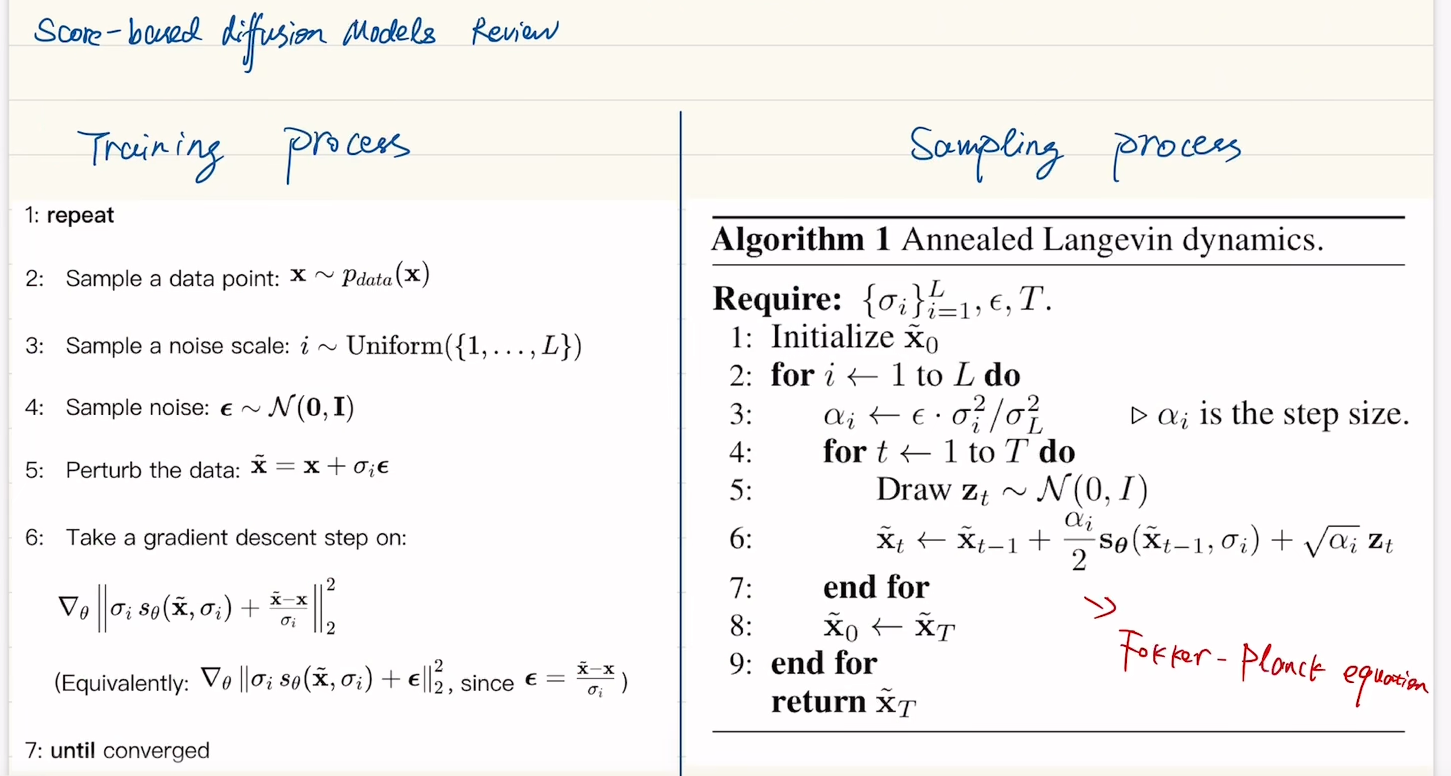
\includegraphics[width=0.7\linewidth]{fig/image.png}
    \caption{score matching}
    % \label{fig:placeholder}
\end{figure}


\section{基于强化学习的扩散模型}
\begin{figure}
    \centering
    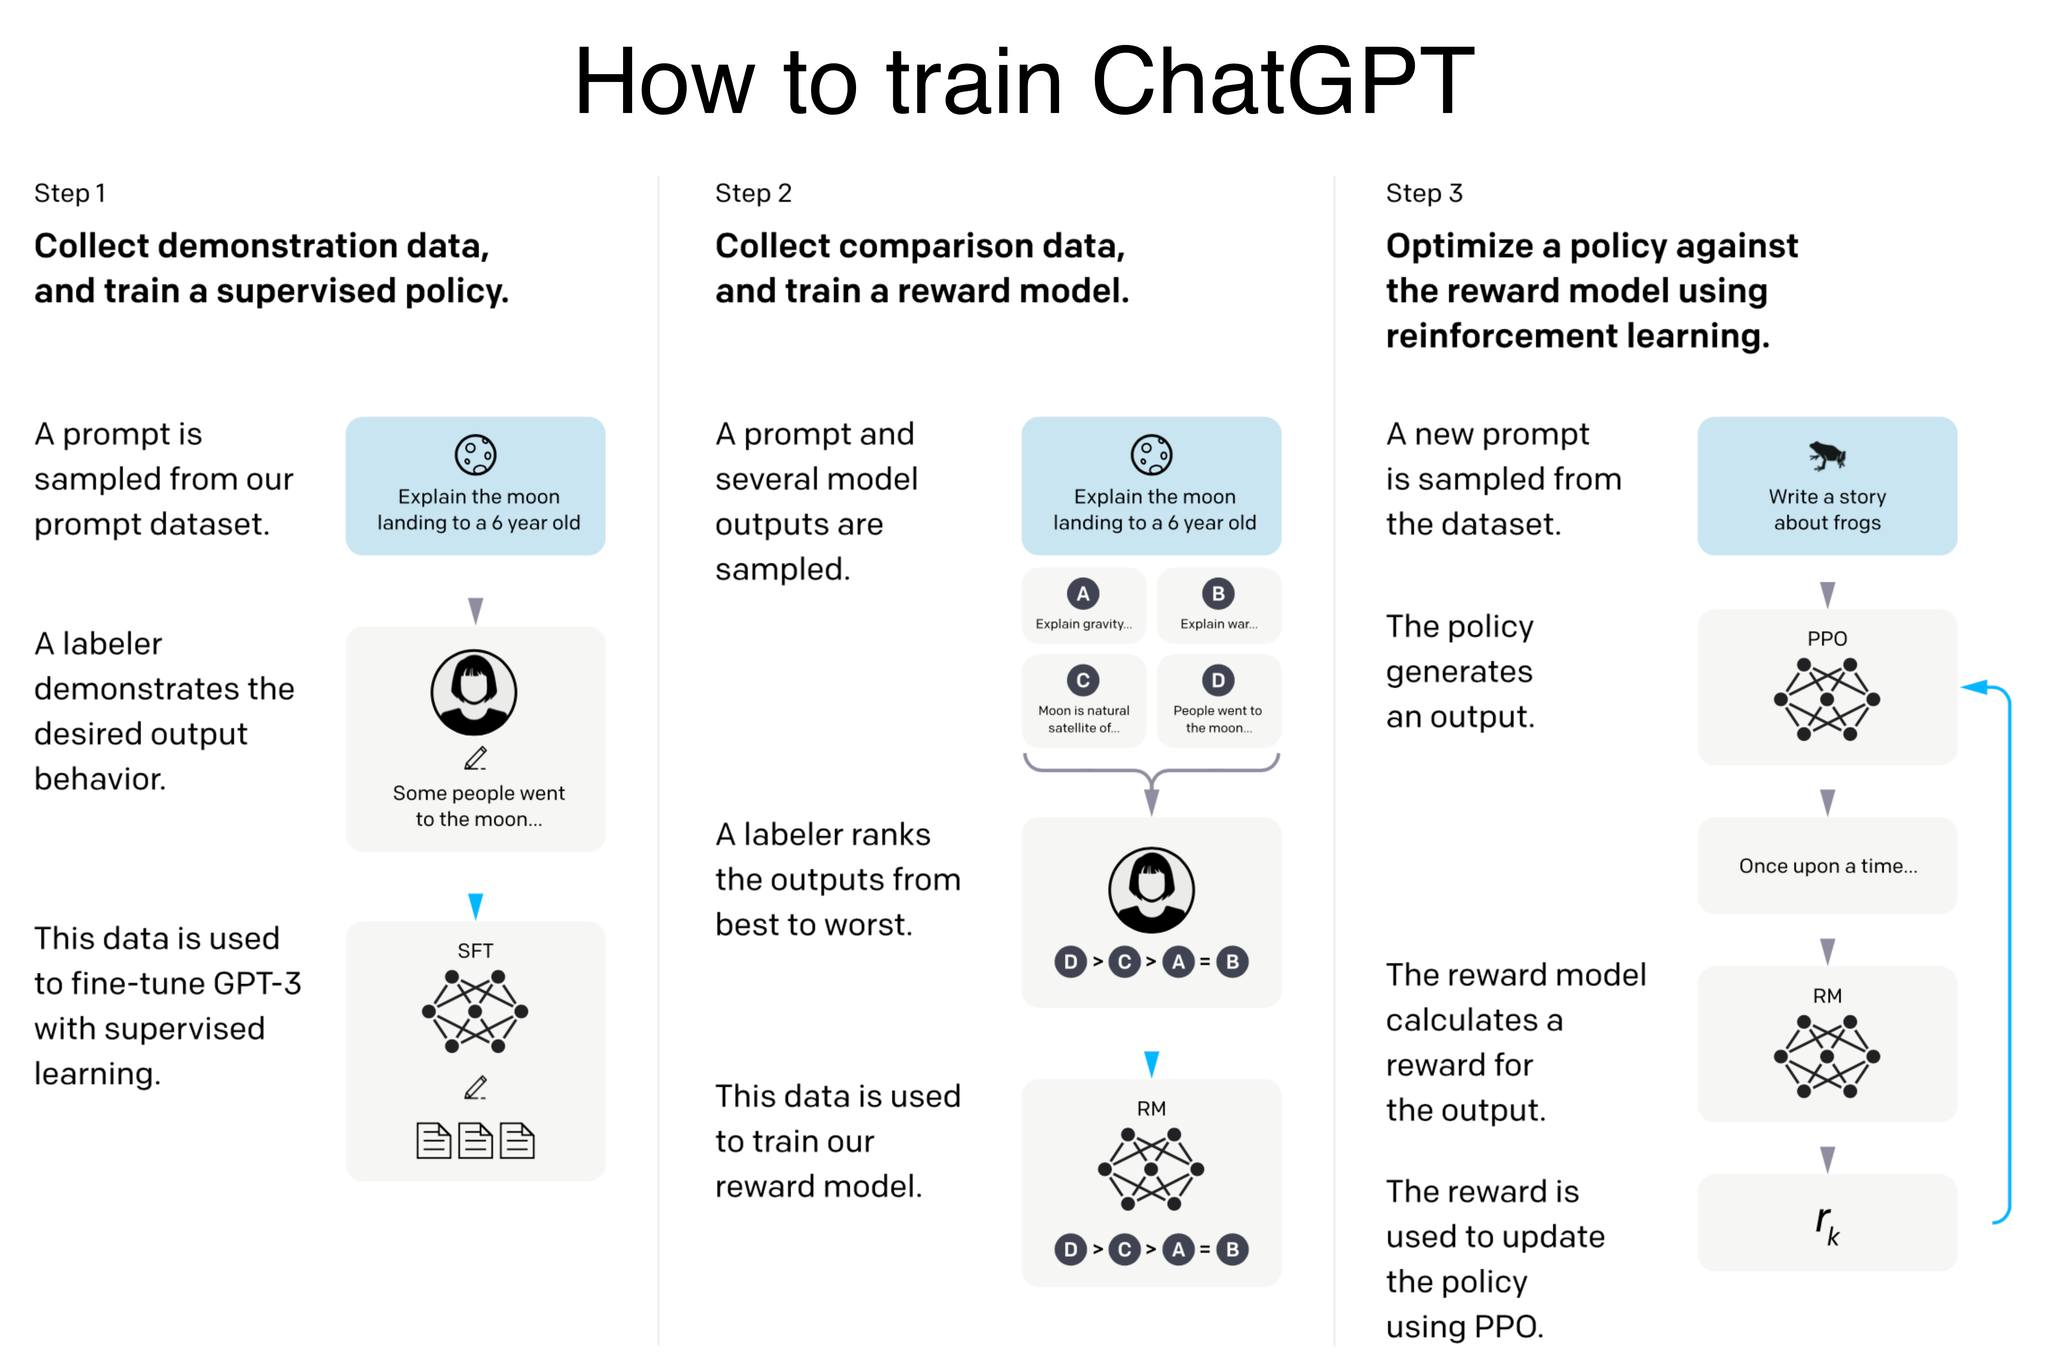
\includegraphics[width=0.8\linewidth]{fig/1.png}
    \caption{RLHF}
    % \label{fig:placeholder}
\end{figure}

%\newpage
%\begin{center}
%{\LARGE \textbf{2025年4月}}
%\end{center}
%% 基础信息框
%\begin{tcolorbox}[colback=yellow!5!white, colframe=yellow!75!black, title=LectureInformation]
%\textbf{Lecture Number: 2} \\
%\textbf{Student: MIStalE} \\
%\textbf{School: Fudan University} \\
%\textbf{Course: Optimization} \\
%\textbf{Date: Fall 2024}
%\end{tcolorbox}
%\section{Newton's Method}
%假设 \( f(x) \) 是 \textit{两次连续可微的} 且 \textit{强凸}。那么可以用以下二次近似对\( f(x_{k+1}) \) 进行描述：
%\[
%f(x_{k+1})\approx f(x_k)+\nabla f(x_k)^T(x_{k+1}-x_k)+\frac{1}{2}(x_{k+1}-x_k)^T\nabla^2f(x_k)(x_{k+1}-x_k)
%\]
%令 \( p = x_{k+1} - x_k \)，我们最小化右边的二次近似得到一个近似的最优解\( x_{k+1} \)：\[
%x_{k+1} = \arg\min_p \left[ f(x_k) + \nabla f(x_k)^T p + \frac{1}{2} p^T \nabla^2 f(x_k) p
%\right] + x_k
%\]
%通过求解上式的最优 \( p \)，我们可以得到：
%\[
%\nabla f(x_k) + \nabla^2 f(x_k) p = 0. \]
%\begin{myanalysis}
%由于 \(\nabla^2 f(x_k)\) 是正定的，它是非奇异的。因此，牛顿法的更新为：\[
%x_{k+1} = x_k - \nabla^2 f(x_k)^{-1} \nabla f(x_k). \]
%\end{myanalysis}
%%	\begin{figure}[H]
%%		\centering
%%		\includegraphics[width=0.6\linewidth]{figure/newton_vs_gd.png}
%%		\caption{Comparison between Newton's method (blue) and the gradient descent
%%			method (black).}
%%		\label{fig:newton_convergence}
%%	\end{figure}
%\begin{mytheorem}
%\label{thm:newton_convergence}
%设 \( f \) 是定义在 \( \mathbb{R}^n \) 上的两次连续可微的函数。假设以下条件成立：\begin{itemize}
%\item \( f \) 是参数为 \( m \) 的强凸函数：存在 \( m > 0 \)，使得对任何\( x \in\mathbb{R}^n \)，有 \( \nabla^2 f(x) \succeq mI \)。
%\item \( \nabla^2 f \) 是 Lipschitz 连续的，参数为 \( L \)：存在\( L > 0 \)，对任何\( x, y \in \mathbb{R}^n \)，有 \( \|\nabla^2 f(x) - \nabla^2 f(y)\| \leq L \|x - y\| \)。\end{itemize}
%设 \( \{x_k\}_{k \geq 0} \) 为牛顿法生成的序列，且 \( x^* \) 是 \( f \) 在\( \mathbb{R}^n\)
%上的唯一最小值。那么对于任意 \( k = 0, 1, \ldots \)，不等式
%\[
%\|x_{k+1} - x^*\| \leq \frac{L}{2m} \|x_k - x^*\|^2
%\]
%成立。此外，如果 \( \|x_0 - x^*\| \leq \frac{m}{L} \)，则有
%\[
%\|x_k - x^*\| \leq \frac{2m}{L} \left( \frac{1}{2} \right)^{2^k}. \]
%\end{mytheorem}
%\section{Damped Newton's Method}
%尽管牛顿法具有快速收敛的特点，但它并不是一个通用的下降方法。在某些情况下，为了使牛顿法更稳定，我们引入一个步长来进行线搜索，从而得到所谓的阻尼牛顿法。以下是阻尼牛顿法的伪代码表示：
%\begin{myalgorithm}
%\begin{algorithm}[H]
%\caption{算法名称}
%\begin{algorithmic}[1]
%%			\Require 目标函数 \( f(x) \)，约束条件 \( x \in X \)，精度阈值 \( \epsilon > 0 \)
%%			\Ensure 最优解 \( x^* \) 和最优值 \( \lambda^* \)
%\State \textbf{Input:} 目标函数 \( f(x) \)，约束条件 \( x \in X \)，精度阈值 \( \epsilon > 0 \)
%\State \textbf{Output:} 最优解 \( x^* \) 和最优值 \( \lambda^* \)
%\State 初始化：选择一个初始值 \( \lambda^{(0)} \in \mathbb{R} \)，设置迭代次数 \( k = 0 \)
%
%\Repeat
%\State \textbf{Step 1:} 求解子问题：
%\[
%x^{(k)} = \arg \max_{x \in X} \bigl\{ f(x) - \lambda^{(k)} g(x) \bigr\}
%\]
%
%\State \textbf{Step 2:} 计算：
%\[
%\phi(\lambda^{(k)}) = \max_{x \in X} \bigl\{ f(x) - \lambda^{(k)} g(x) \bigr\}
%\]
%
%\State \textbf{Step 3:} 更新：
%\[
%\lambda^{(k+1)} = \frac{f(x^{(k)})}{g(x^{(k)})}
%\]
%
%\State 更新迭代次数： \( k \gets k + 1 \)
%
%\Until \( \phi(\lambda^{(k)}) < \epsilon \)
%
%\State 输出最优解：\( x^* = x^{(k)} \)，最优值：\( \lambda^* = \lambda^{(k)} \)
%\end{algorithmic}
%\end{algorithm}
%\end{myalgorithm}
%
%\begin{myremark}
%牛顿法在大规模优化问题中可能需要大量的存储和计算资源，这时我们可以利用稀疏矩阵的特性或使用共轭梯度法来求解线性系统，从而提高计算效率。
%\end{myremark}
%\section{总结}
%\begin{tcolorbox}[colback=yellow!5!white, colframe=yellow!75!black, title=总结]
%牛顿法是求解强凸函数最优化问题的有效方法，在初始点足够接近最优解时具有二次收敛的性质。然而，其计算复杂度较高，特别是在 Hessian 矩阵稠密或规模较大时。通过引入步长，阻尼牛顿法增强了牛顿法的鲁棒性，使其在较远的初始点也能稳定收敛。\end{tcolorbox}
\end{document}




